\documentclass{article}
\usepackage[utf8]{inputenc}
\usepackage{import}
\usepackage[subpreambles=true]{standalone}
\usepackage{graphicx}
\usepackage{amsmath}
\usepackage{amsfonts}
\usepackage{amssymb}
\usepackage{mathrsfs}
\usepackage{enumerate}
\usepackage{fancyhdr}
\usepackage[colorlinks=true,linkcolor=black,anchorcolor=black,citecolor=black,filecolor=black,menucolor=black,runcolor=black,urlcolor=blue]{hyperref}
\usepackage[margin=1.75in]{geometry}
\usepackage{algorithm, algpseudocode}
\usepackage{tikz}
\usepackage{ulem}
\usetikzlibrary{backgrounds, calc, positioning}

\tikzstyle{arr}=[fill=white, draw=black, shape=rectangle, minimum width = {width("100")}]
\tikzstyle{cir}=[fill=white, draw=black, shape=circle]

\begin{document}
%%%%%%%%%%%%%%%%%%%%%%%%%%%%
%%     Chapter Content    %%
%%%%%%%%%%%%%%%%%%%%%%%%%%%%
\section{Heap Sort}
\rule{\textwidth}{1pt}
\subsection{Pseudocode}
\begin{algorithm}
\caption{Heap Sort}
\begin{algorithmic}[1]
\Procedure{Heapsort}{$A, n$}\Comment $A$ is a list and $n$ is $A$'s size
	\For{$r = \lfloor n/2\rfloor$ \textbf{down to} $1$}\Comment Create Heap
		\State\Call{sift}{$r,n$}
	\EndFor
	\State
	\For{$m=n$ \textbf{down to} $2$}\Comment Finish Sort
		\State $A[1]\leftrightarrow A[m]$
		\State\Call{sift}{$1,m-1$}
	\EndFor
\EndProcedure
\Statex
\Procedure{sift}{$p, m$}\Comment $p$ is the root and $m$ is the size of the list
	\State $c\leftarrow 2p$
	\While{$c\leq m$}
		\If{$c<m$}
			\If{$A[c+1]>A[c]$} 
				\State $c\leftarrow c+1$
		\EndIf
		\EndIf
		\State
		\If{$A[c]>A[p]$}
			\State $A[p] \leftrightarrow A[c]$
			\State $p\leftarrow c$
			\State $c\leftarrow 2p$
		\Else
			\State exit while loop
		\EndIf
	\EndWhile
\EndProcedure
\end{algorithmic}
\end{algorithm}

\subsection{Create Heap}
A Heap is a binary tree where every value is larger than its children.
Equivalently its descendants. For the purposes of this class will we require
that all binary trees are full binary trees.
\begin{center}
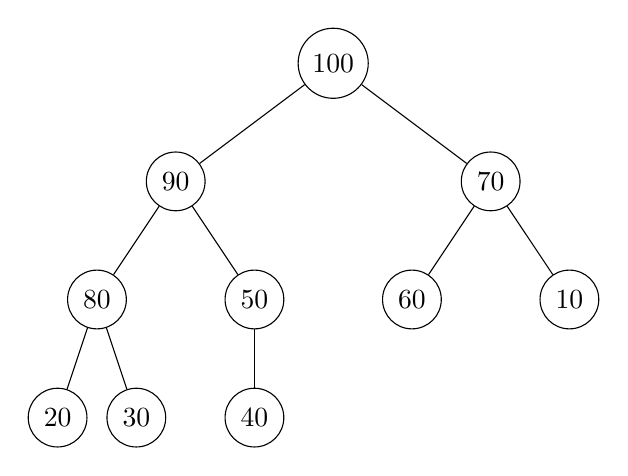
\begin{tikzpicture}
	\node[style=cir] (1) at (0,0) {100};
	\node[style=cir] (2) at (-2, -1.5) {90};
	\node[style=cir] (3) at (2, -1.5) {70};
	\node[style=cir] (4) at (-3, -3) {80};
	\node[style=cir] (5) at (-1, -3) {50};
	\node[style=cir] (6) at (1, -3) {60};
	\node[style=cir] (7) at (3, -3) {10};
	\node[style=cir] (8) at (-3.5, -4.5) {20};
	\node[style=cir] (9) at (-2.5, -4.5) {30};
	\node[style=cir] (10) at (-1, -4.5) {40};

	\draw (2) to (1);
	\draw (3) to (1);
	\draw (4) to (2);
	\draw (5) to (2);
	\draw (6) to (3);
	\draw (7) to (3);
	\draw (8) to (4);
	\draw (9) to (4);
	\draw (10) to (5);
\end{tikzpicture}	
\end{center}
The traditional way of creating a heap is to insert at
the end of the array and sift up. Robert Floyd created a better algorithm for creating
the heap. Treat the tree as a recursive heap: each parent is the parent of 2 heaps,
and sift from the bottom up. Create heap on left, create heap on right, then sift
root down, and move up a level. 
\subsubsection*{Heap Creation Analysis}
In a binary tree, most nodes are near the bottom, so when doing the bottom up technique,
most of the work is done at the bottom. The number of comparisons can be calculated like so,
\begin{align*}
	\frac{n}{2}\cdot 0 + \frac{n}{4}\cdot 2 + \frac{n}{8}\cdot 4 + \cdots &= \\
	&= n\left[\frac{1}{2} + \frac{2}{4} + \frac{3}{8} + \cdots\right]
\end{align*}
Note that $\left[\frac{1}{2} + \frac{2}{4} + \frac{3}{8} + \cdots\right]$ can be written as so,
\begin{align*}
	\frac{1}{2} + \frac{1}{4} + \frac{1}{8} + \cdots &= 1 \\
	\frac{1}{4} + \frac{1}{8} + \cdots &= \frac{1}{2} \\
	\frac{1}{8} + \cdots &= \frac{1}{4}
\end{align*}
Which all together becomes
$$1 + \frac{1}{2} + \frac{1}{4} + \cdots = 2$$
So Heap creation does $2n$ comparisons.

\subsection{Finish Sort}
After heap creation we then sort it,
\begin{itemize}
	\item Put root node at the bottom of the array (it must be the largest element) so it goes to end
	of the sorted array.

	\item Then take the bottom right hand leaf and move to a temporary space.
	
	\item Then sift, reordering the tree and put the temporary leaf in its proper spot.
	
	\item Repeat until all elements are sorted.
\end{itemize}
\subsubsection*{Heap Sort Analysis}
Each level has two comparisons, child and temporary. There are $\approx \lg n$ levels,
so the total comparisons for a sift is $\approx 2\lg n$. This is done for each element
in the tree so worst case we get $\approx 2n\lg n$. But heap shrinks upon each iteration
(it removes an element) so we take the sum from $0$ to $n-1$.
\begin{align*}
	\sum_{i=0}^{n-1} 2\lg(i+1) &\approx 2\sum_{i=1}^{n} \lg i \\
	&= 2[\lg 1 + \lg 2 + \lg 3 + \cdots + \lg n] \\
	&= 2\lg (1\times 2\times 3\times\cdots\times n) \\
	&= 2\lg (n!) \\
	&= 2\lg\left[\left(\frac{n}{e}\right)^n \cdot \sqrt{2\pi n}\right] \\
	&\approx 2\left[n\lg\left(\frac{n}{e}\right) + \frac{\lg (2\pi n)}{2}\right] \\
	&= 2n\lg n - 2n\lg e + \lg n + \lg (2\pi) \\
	&= 2n\lg n + O(n)
\end{align*}
From this we see that even while the tree shrinks, it does not shrink fast enough to make
some notable difference. We are still doing $2n\lg n$ comparisons.

\subsection{Implementation}
\begin{figure}[H]
	\centering
	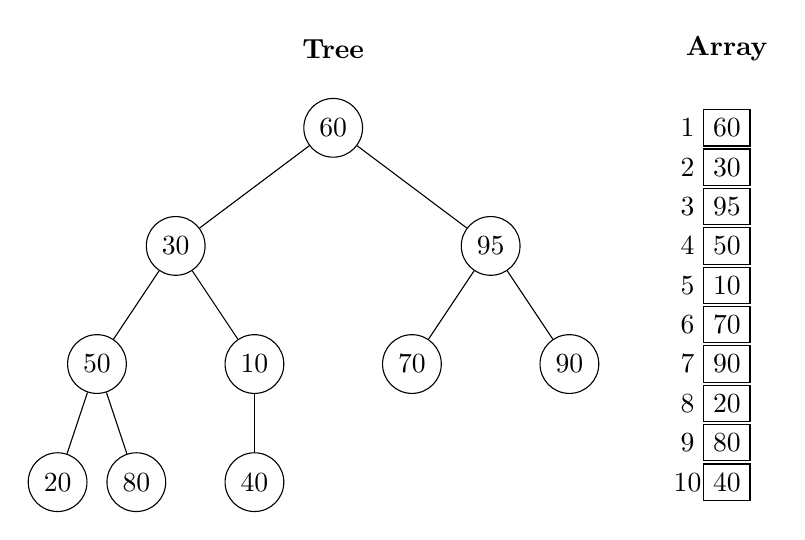
\begin{tikzpicture}
		\node[style=cir] (1) at (0,0) {60};
		\node[style=cir] (2) at (-2, -1.5) {30};
		\node[style=cir] (3) at (2, -1.5) {95};
		\node[style=cir] (4) at (-3, -3) {50};
		\node[style=cir] (5) at (-1, -3) {10};
		\node[style=cir] (6) at (1, -3) {70};
		\node[style=cir] (7) at (3, -3) {90};
		\node[style=cir] (8) at (-3.5, -4.5) {20};
		\node[style=cir] (9) at (-2.5, -4.5) {80};
		\node[style=cir] (10) at (-1, -4.5) {40};
	
		\draw (2) to (1);
		\draw (3) to (1);
		\draw (4) to (2);
		\draw (5) to (2);
		\draw (6) to (3);
		\draw (7) to (3);
		\draw (8) to (4);
		\draw (9) to (4);
		\draw (10) to (5);

		\node[style=arr] (11) at (5, 0) {60};
		\node[style=arr] (12) at (5, -.5) {30};
		\node[style=arr] (13) at (5, -1) {95};
		\node[style=arr] (14) at (5, -1.5) {50};
		\node[style=arr] (15) at (5, -2) {10};
		\node[style=arr] (16) at (5, -2.5) {70};
		\node[style=arr] (17) at (5, -3) {90};
		\node[style=arr] (18) at (5, -3.5) {20};
		\node[style=arr] (19) at (5, -4) {80};
		\node[style=arr] (20) at (5, -4.5) {40};

		\node (21) at (4.5, 0) {1};
		\node (22) at (4.5, -.5) {2};
		\node (23) at (4.5, -1) {3};
		\node (24) at (4.5, -1.5) {4};
		\node (25) at (4.5, -2) {5};
		\node (26) at (4.5, -2.5) {6};
		\node (27) at (4.5, -3) {7};
		\node (28) at (4.5, -3.5) {8};
		\node (29) at (4.5, -4) {9};
		\node (30) at (4.5, -4.5) {10};

		\node at (0,1) {\textbf{Tree}};
		\node at (5,1) {\textbf{Array}};
	\end{tikzpicture}
	\caption[]{Use an array to implement a tree.}
	Node has index $i$, Left child is $2i$, Right child is $2i+1$, and Parent is $\lfloor \frac{i}{2}\rfloor$.
\end{figure}
\subsubsection*{Create}
The first parent is at index $\lfloor \frac{n}{2}\rfloor$. Start there and sift down during
heap creation. Siblings can be reached by adding or subtracting 1. The result is a created heap.

\subsubsection*{Finish}
To finish the sort we push bottom into tmp first, then move heap root into the bottom most spot.

\subsection{Optimization}
As Heapsort stands, the result is worse than merge sort. $\Theta(2n\lg n)$ vs $\Theta(n\lg n)$ shows
us that much. We compare tmp against both children and this doubles our total number of comparisons.
Instead we can sift the hole left by the root down to the bottom in $\lg n$ comparisons.
Then put tmp in the hole and sift it back into position.
It follows then that we give up $2n$ comparisons on average.
Further optimization can be achieved by binary searching up. This gives Heapsort
$n\lg n + n\lg (\lg n) = \Theta (n\lg n)$ performance.

\end{document}